\chapter{F\'azis\'atalakuls\'asok oszt\'alyoz\'asa, folyad\'ek--g\'az \'atalakul\'as, van der Waals elm\'elet, univerzalit\'as} 
 
 \section{Fázisátalakulások osztályozása}
  
  A fázisátalakulásoknak nehezen adható meg jó definíciója, olyan általános jelenségről van szó.
   Fázisátalakulás akkor történik, ha a termodinamikai mennyiségek nem analitikusan változnak.
   Egy fázisban található egy rendszernek egy része, ha az adott részen belül minden termodinamikai mennyiség analitikusan változik.
  
  $X$ egy makroszkopikus mennyiség, amitől függ a termodinamikai potenciál: $\phi(X)$.
   Ekkor $X$ eloszlása: $P(x)\sim e^{-\beta\phi(x)}$. $P$ éles eloszlás, így a legvalószínűbb és az átlagos $X$ érték megegyezik.
   Keressük meg $\phi(X)$ minimumát $X$ szerint, ott lesz a legvalószínűbb állapot.
   Ennek stabilitását a $\phi(X)$ második derivátjának előjele dönti el. 
  
  \paragraph{Elsőrendű átalakulások}
  
   A termodinamikai potenciál minimumának a helye változik meg, stabil $\rightarrow$ metastabil átalakulás történik.
   Ekkor a termodinamikai potenciál első deriváltja mutat nemanalitikus viselkedést.
   Ezt mutatja \aref{fig:B09-elsorend}. ábra.
   Jól láthatjuk, hogy az egyensúlyi $m$ értéke ($F$ globális minimumának a helye) az átalakulásnál ugrik. 
   
   \begin{figure}[ht!]
    \centering
    \subfloat[$H<0$\label{fig:B09-e1}]{\includegraphics[width= 0.3\textwidth]{./B09tetel/elsorendu2_Ising}} \hspace{6pt}
    \subfloat[$H=0$\label{fig:B09-e2}]{\includegraphics[width= 0.3\textwidth]{./B09tetel/elsorendu1_Ising}} \hspace{6pt}
    \subfloat[$H>0$\label{fig:B09-e3}]{\includegraphics[width= 0.3\textwidth]{./B09tetel/elsorendu0_Ising}} 
    \caption{
     $T<\TC$ esetben a mágneses tér itt balról jobbra nő, és közben előjelet vált.
   Kezdetben a véges nagyságú $m$ állapot volt stabil, majd a tér növelésével elérünk egy olyan állapotot, hogy az $m=-m_0$ és az $m=m_0$ állapot lesz is ugyanúgy stabil.
   Ez a koegzisztencia állapota.
   A tér további növelésével az $m>0$ állapot lesz a stabil. 
    }\label{fig:B09-elsorend}
   \end{figure}
   
   A fázishatáron a két fázis egymással egyensúlyban van, így igaz, hogy $G_1=G_2$, hol $G$ az egyik és a másik fázis szabadentalpiája.
   A fázishatáron való elmozdulásnál:
   \al{
    \dd G_1&=\dd G_2\\
    V_1\dd p-S_1\dd T&=V_2\dd p-S_2\dd T\\
    \der{p}{t}&=\frac{S_2-S_1}{V_2-V_1}=\frac{1}{T}\frac{\Delta H}{\Delta V},
   }  
   ahol $\Delta V$ a két fázis közötti fajlagos térfogatkülönbség, és $\Delta S$ a fajlagos entrópiakülönbség.
   Ez a Clausius--Clapeyron-egyenlet.
   Ha $\Delta V$ és/vagy $\Delta H$ ugrik, akkor elsőrendű a változás.
  
  \paragraph{Másodrendű átalakulás} 
  
   Itt stabil $\rightarrow$ stabilitási határ $\rightarrow$ instabil átalakulás történik meg.
   Ekkor az hőmérséklet változtatásával a kezdetben stabil állapot instabillá válik, és a termodinamikai potenciál minimumhelye máshova kerül.
   Egy ilyen folyamatot \aref{fig:B09-masodrend}. ábra mutat.
  \begin{figure}[ht!]
   \centering
   \subfloat[$T>T_\text{C}$\label{fig:B09-m1}]{\includegraphics[width= 0.3\textwidth]{./B09tetel/masodrendu2}} \hspace{6pt}
   \subfloat[$T=T_\text{C}$\label{fig:B09-m2}]{\includegraphics[width= 0.3\textwidth]{./B09tetel/masodrendu1}} \hspace{6pt}
   \subfloat[$T<T_\text{C}$\label{fig:B09-m3}]{\includegraphics[width= 0.3\textwidth]{./B09tetel/masodrendu0}} 
   \caption{A hőmérséklet balról jobbra csökken, az egyensúlyi mágnesezettség (minimumhely) pedig folytonosan változik.}\label{fig:B09-masodrend}
  \end{figure}
  
  A Clausius--Clapeyron-egyenlet itt is helytálló, azonban itt a $\Delta V$ és a $\Delta S$ is folyamatosan változik, így a jobb oldal átmegy egy deriválásba és az egyenlet pedig megegyezik az egyik Maxwell-relációval.
  
  \section{Folyadék--gáz átalakulás}\label{ss:B09-vdW}
   
   A folyadék--gáz átalakulás leírásához a van der Waals-elméletet fogjuk használni.
   Célunk az, hogy az ideális gáz állapotegyenletén túl szeretnénk lépni, figyelembe szeretnénk venni a részecskék kölcsönhatását. van der Waals bevezet egy szabadenergia-sűrűséget, melyből lehezethető az állapotegyenlet:
   \al{
    p=\frac{N\kB T }{V-bN}-a\frac{N^2}{V^2}.
   }
   A $b$ paraméterre gondolhatunk úgy, mint a részecskék térfogatára, illetve $a$-ra úgy, mint a részecskék közötti kölcsönhatásra.
   A két anyagi paraméter hőmérsékletfüggetlen.
   Az ideális esethez képest a nyomás a $b$ paraméter miatt megnő, hiszen a részecskék is helyet foglalnak ezenúl, az $a$ paraméter miatt pedig csökken, a részecskék között vonzó kölcsönhatás van. 
   
   A $p(V)$ függvénynek inflexiós pontja van egy jól meghatározott $T_\text{C}$, $T_\text{C}$, $p_\text{C}$ értéknél.
   Ekkor $\pder{p}{V}=0$ és $\pder{^2p}{V^2}=0$.
   Az állapotegyenletet és ezt a két összefüggést felhasználva:
   \al{
    &V_\text{C}=3b&
    &p_\text{C}=\frac{a}{27b^2}&
    &k_\text{B}T_\text{C}=\frac{8a}{27b}.
   }
   Az állapotegyenlet anyagfüggetlenné tehető a redukált mennyiségek bevezetésével:
   \al{
      &\bar{V}=\frac{V}{V_\text{C}}&
      \bar{p}&=\frac{p}{p_\text{C}}&
      &\bar{T}=\frac{T}{T_\text{C}}\\
      &&\left(\bar{p}+\frac{3}{\bar{V}}\right)&\left(3\bar{V}-1\right)=8\bar{T}&&
   }
   Az egyenlet megoldásait mutatja \aref{fig:B09-vdW}. ábra.
   Az állapot ezen alakja univerzális, nem függ attól, hogy milyen anyagra írtuk fel.
   Két anyag megfelelő állapotban van, ha a redukált mennyiségei megegyeznek.
   Ekkor a fenti egyenlet fogja mind a kettőnek a viselkedését leírni, függetlenül attól, hogy milyen rendszerekről van szó.
   
   \begin{figure}[ht!]
    \centering
    \subfloat[\label{fig:B09-vdW1}]{\includegraphics[width= 0.3\textwidth]{./B09tetel/direktvdW}} \hspace{6pt}
    \subfloat[\label{fig:B09-vdW2}]{\includegraphics[width= 0.3\textwidth]{./B09tetel/Mxkonstr}} \hspace{6pt}
    \subfloat[\label{fig:B09-vdW3}]{\includegraphics[width= 0.3\textwidth]{./B09tetel/valodivdW}} 
    \caption{Az (a) ábrán láthatóak van der Waals állapotegyenlet megoldásai.
   A narancssárga görbe mutatja, hogy hol válik instabil az állapot, a görbe alatti területen nem fizikai állapotok vannak, ugyanis $-\pder{p}{V}\sim\kappa^{-1}<0$.}. \label{fig:B09-vdW}
   \end{figure}
   
   \paragraph{Maxwell-konstrukció}
   
    A nem fizikai állapotok helyett valamilyen fizikai megoldást kell találni.
   Ezeket a Maxwell-konstrukció adja meg.
   A szabadentalpia: $G=\intl{}{}\dd p\, V(p)$, melyet \aref{fig:B09-Gp}. ábra mutat.
   Az izotermán haladva az $ABCDEF$ útvonalon haladnánk végig.
   Az alapgondolat az, hogy a rendszer akkor van egyensúlyban, ha a szabadentalpia minimális, ez pedig az $ABEF$ útvonalon áll fenn.
   Az átalakulásnak megfelelő nyomáson a szabadentalpia minimuma megtörik.
   Végülis az átalakulás állandó nyomáson történik, a $BCDE$ hurok nem valósul meg, a szabadentalpia az $ABEF$ útvonalon változik.
   
    \begin{figure}[ht!]
    \centering
    \subfloat[$T>T_\text{C}$\label{fig:B09-Gp}]{%
     \begin{tikzpicture}
     \draw[-latex] (0,0) -- (5,0) node[below right] {$p$};
     \draw[-latex] (0,0) -- (0,4) node[above left] {$G$};
     \draw[line width=1pt] (0.5,0.5) node[below right=-4pt] {$A$} .. controls (1,1.1) and (2,2.2) .. (3,3) node[above right=-4pt] {$C$};
     \draw[line width=1pt] (3,3) .. controls (2.5,2.8) and (2.3,2.7) .. (1.8,2.3);
     \draw[line width=1pt] (1.8,2.3) node[below left=-4pt] {$D$} .. controls (2,2.45) and (3.6,2.95) .. (4.5,3) node[below=-2pt] {$F$};
     \node[below=-2pt] at (3,2.5) {$B=E$};
     \end{tikzpicture}
    }
    \hspace{6pt}
    \subfloat[$T>T_\text{C}$\label{fig:B09-specatal}]{%
     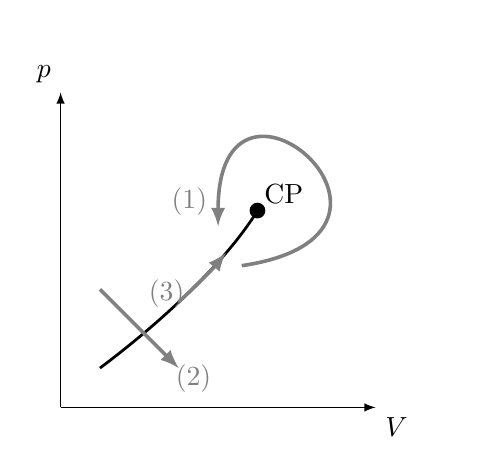
\begin{tikzpicture}
      \draw[-latex] (0,0) -- (4,0) node[below right] {$V$};
      \draw[-latex] (0,0) -- (0,4) node[above left] {$p$};
      \draw[line width=1pt] (0.5,0.5) .. controls (1.5,1.25) and (2.2,2.0) .. (2.5,2.5);
      \fill (2.5,2.5) circle (0.1) node[above right=-1pt] {CP};
      \draw[-latex,gray,line width=1.3pt] (0.5,1.5) -- (1.5,0.5) node[below right=-5pt] {$(2)$};
      \draw[-latex,gray,line width=1.3pt] (2.3,1.8) .. controls (5,2.2) and (2,4.8) .. (2,2.3) node[above left ] {$(1)$};
      \draw[-latex,gray,line width=1.3pt] (1.5,1.34) node[above left=-6pt]{$(3)$} .. controls (1.6,1.43) and (1.9,1.72) .. (2.1,1.965);
     \end{tikzpicture}
    }
    \caption{A szabadentalpia a nyomás függvényében (a), illetve speciális átalakulások a kritikus pont körül (b).}\label{fig:B09-gpspecatal}
   \end{figure}
    
   \paragraph{A kritikus pont körüli átalakulások} Speciális átalakulásokat mutat \aref{fig:B09-specatal}. ábra:

   \begin{enumerate}
    \item[(1)] Ekkor nem haladunk át fázishatáron, így a gőz/gáz/folyadék között nem látjuk sosem a különbséget.
   Ezen az úton nem történik fázisátalakulás, minden termodinamikai mennyiség analitikusan változik.
    \item[(2)] Áthaladunk a fázishatáron, elsőrendű fázisátalakulás történik.
   A fázishatáron különbséget látunk a folyadék és a gőz között, az egyik fázis moláris térfogata jóval nagyobb, mint a másiké. 
    \item[(3)] A fázishatáron haladva látjuk a különbséget a gőz és a folyadék között (a moláris térfogat különbözik).
   A kritikus pont felé haladva a sűrűségkülönbség csökken, és a kritikus pontban nullává válik.
   Ahogy áthaladunk a kritikus ponton, már csak egy fázist látunk.
   Mivel a $\Delta V$ folytonosan vált nullává, ez az átalakulás folytonos: másodrendű.
   \end{enumerate}

  \section{Univerzalitás}
   
   Lásd \aref{ss:B10-univerzalitas}. fejezetben.
